\section{Methods}
\label{sec:methods}

%\subsection{Study design}

The proposed estimation model is summarized in Figure \ref{speed_system}. The data was collected from body-mounted \gls{imu}s and \gls{gps} devices. Then, the data was time-synchronized, preprocessed, and split in windows for time- and frequency-domain feature extraction. Subsequently, "feature set"s were defined as the extracted features from one \gls{imu} or a combination of \gls{imu}s. To decrease the number of features used in the estimation model, the optimal group of features was identified using a feature selection method for each feature set. Next, estimation models were trained using popular machine learning techniques in the literature \cite{Bouwman2020,Zhou2020}, which were \gls{svm}  \cite{cortes_1995_supportvector}, \gls{gpr} \cite{carledwardrasmussen_2008_gaussian}, decision tree \cite{quinlan_1986_induction}, \gls{gbt} \cite{friedman_2002_stochastic,SUT201115534}, and random forest \cite{breiman_2001_random}. Finally, the accuracy of the models were compared.

\begin{figure}[htbp]
\centering
\includegraphics[width=\linewidth]{chapters/Speed/figures/Untitled_HQ.png}
\caption{A summary of the model training procedure.}
\label{speed_system}
\end{figure}

\subsection{\gls{imu} Data Collection}
Considering that different horse breeds exhibit biomechanically distinct characteristics and display varying motion patterns across different gaits \cite{faber,CANO2001147,Robilliard187}, we incorporated motion data from two distinct horse breeds and multiple gaits, including walk, trot, tölt, pace, and canter, in order to develop a comprehensive estimation model. The data used in this study was obtained from various research projects. In one study, data was collected from fifteen Icelandic horses, ridden at walk, trot, tölt, pace, and canter to study the biomechanical properties of different gaits \cite{gunnarsson_2018_objective}. In another study, twenty-five Franches-Montagnes horses were walked and trotted in hand to study gaits and phenotype-genotype associations \cite{franches}. In both studies, horses were equipped with an identical gait analysis system (EquiMoves), which comprised seven ProMove-mini \gls{imu}s (Inertia Technology B.V., Enschede, The Netherlands) (tri-axial accelerometer and tri-axial gyroscope) \cite{456,articsasasasle} on poll, withers, sacrum, and the lateral aspect of all four limbs (cannon bone). \gls{imu} sensors were set to a sampling rate of 200 Hz. Figure \ref{fig:speed_IMUplacement} demonstrates the \gls{imu} locations and orientations on the body of a participant horse. Horses with a known history of lameness or presenting any clear sign of lameness during the measurements were excluded from this study.

As demonstrated in Figure \ref{fig:speed_IMUplacement}, the three axes of rotation for the sacrum, withers, and poll \gls{imu}s were x,y, and z, which were defined in the order as longitudinal axis, mediolateral axis, and vertical axis. For limbs, the x, y, and z-axis were aligned to the limb (longitudinally), retraction/protraction angle axis, and abduction/adduction angle axis, respectively \cite{456}.  

\begin{figure}[htb]
\centering
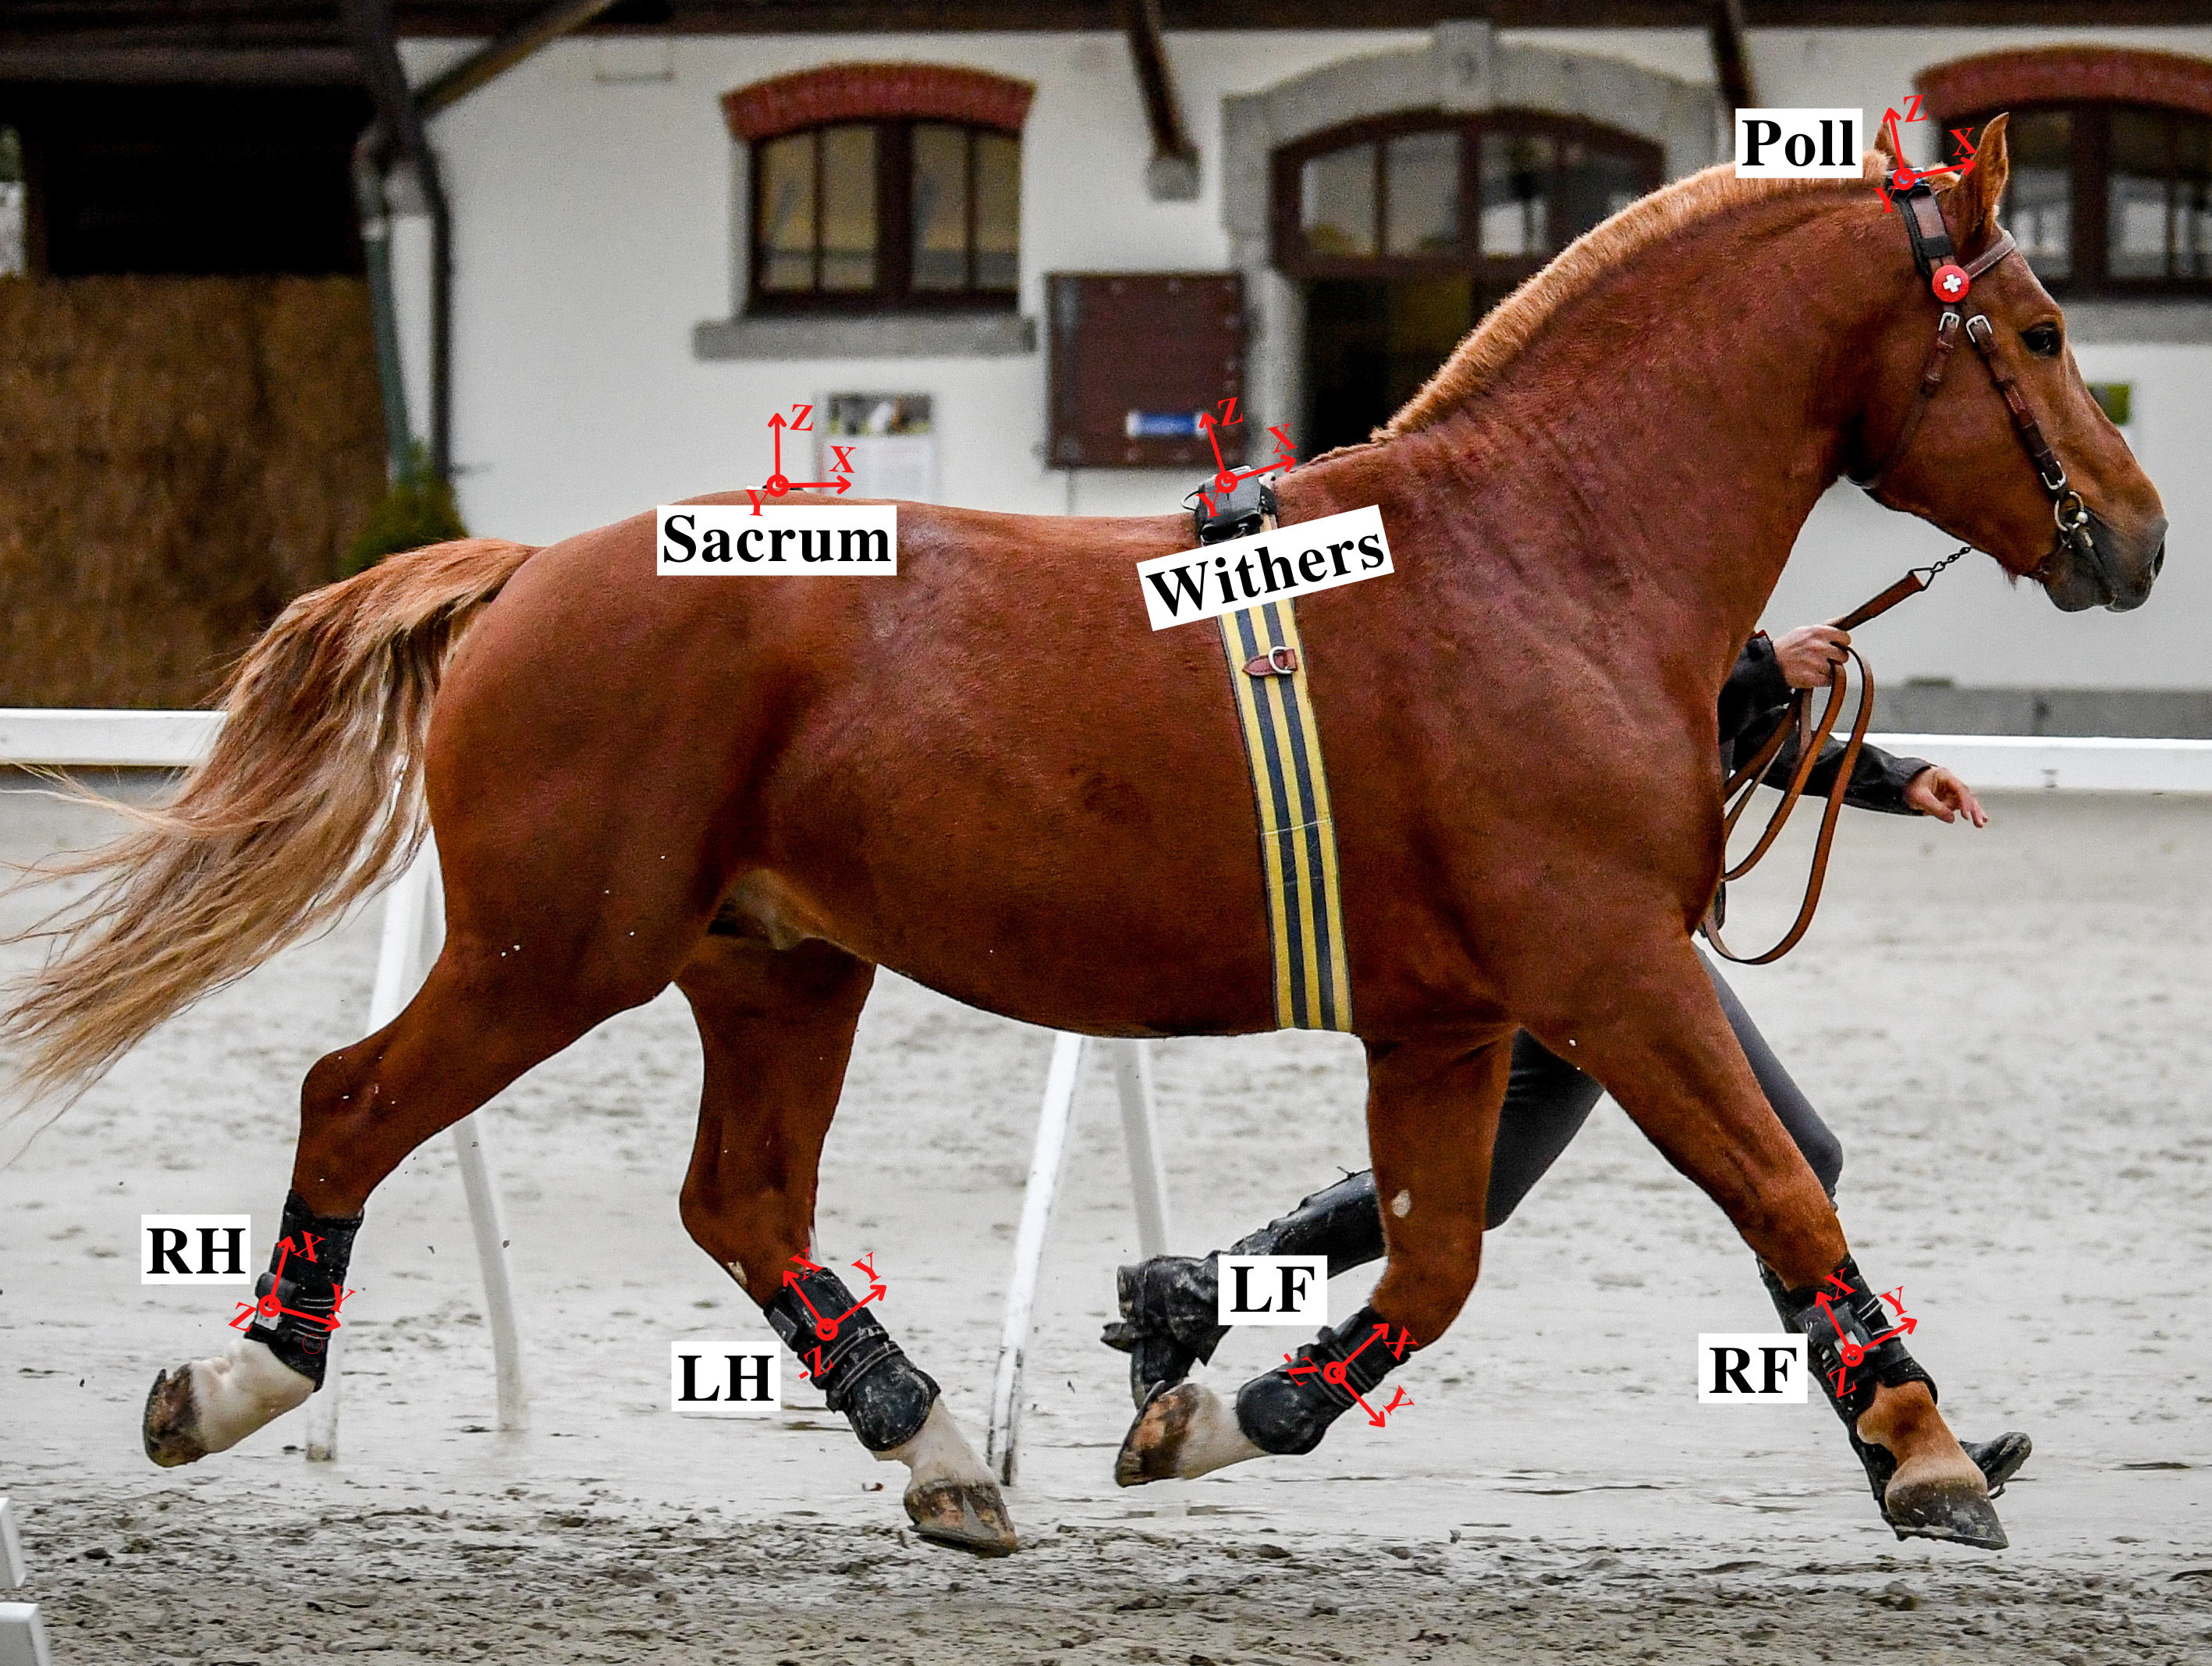
\includegraphics[width=.95\linewidth]{chapters/Speed/figures/Sacrum_HQ.png}
\caption{\gls{imu}s locations and orientations on horse body. {RF: right front limb, LF: left front limb, RH: right hind limb, LH: left hind limb}.  {Photographed by Christelle Althaus.}}
\label{fig:speed_IMUplacement}
\end{figure}

\subsection{\gls{gps} Data Collection}
\label{sec:gpsvalsection}

The sacrum \gls{imu} contained a \gls{gps} module (Hornet ORG14xx, OriginGPS Ltd., Airport City, Israel) for the measurement of Icelandic horses, while for Franches-Montagnes horses, the \gls{gps} module was embedded in the withers \gls{imu}. The sacrum and withers were selected for \gls{gps} placement since they are the clearest points of the horse's body for receiving satellite signals. Therefore, the measurements were performed outdoors. The \gls{gps} sampling configuration was set to 5 Hz. 

The \gls{gps} module has been designed to accurately measure the speed (less than 0.01~m/s error for speed value of 30 m/s) using the Doppler shift method \cite{hornet}. To confirm the accuracy, the module was tested and validated for outdoor speed measurement prior to this study. A report is provided from the validation study and the outcome in the following:

\vspace{3mm}
\noindent\textbf{\gls{gps} validation study}

The \gls{gps} device used in this study had not been validated in scientific papers. Thus, a validation study was proposed prior to the main study to evaluate the sensor accuracy in speed calculation. Afterward, the speed data from the \gls{gps} sensor was exploited as ground truth for building the speed estimation model using \gls{imu} data and machine learning algorithms.

In general, velocity can be calculated by dividing the distance ($\Delta x$) by exceeded time ($\Delta t$). Specifically, the output velocity is the average velocity or the speed that a particle needs to travel $\Delta x$ in $\Delta t$. To calculate the instant velocity or the velocity at an exact sample time, the derivative of the position-time equation should be calculated. However, it is practically impossible to define a time-based equation for a real-world particle position, and as a result, calculating the instant velocity is unreachable. In this study, we tried to minimize the time difference as small as allowed by \gls{gps} device data frequency to be able to calculate velocity on more time samples. Since the output was not instant velocity, in the following, the output velocity is called “near-instant velocity”.

ProMove-mini \gls{imu}, was selected for this study, which contained a \gls{gps} sensor. This \gls{gps} sensor is capable of outputting data in 1 and 5 Hz frequencies. In order to have a near-instant velocity, a 5 Hz frequency was selected for the experiment. In other words, the \gls{gps} output a speed sample every 0.2 seconds ($\Delta t$=0.2 s) using the Doppler effect technique. 

To validate the \gls{gps} sensor for measuring velocity on 5 Hz frequency, a ground truth with the same frequency was required. High-speed cameras have been used in a number of studies for horse speed measurement \cite{fredricson_1980_the,ratzlaff_1985_the}. Therefore, GoPro Hero 5 (GoPro, Inc., San Mateo, CA, USA) was selected for this purpose. This camera has been used for scientific purposes in multiple studies \cite{8036783,10.1371/journal.pone.0212319,SUN2017319}. This camera is capable of recording video in 240 frames per second, which is higher than the \gls{gps} data collection frequency (240 frames per second compared to 5 samples per second). In this study, the camera was set to record in 240 frames per second and linear mode (preventing the video footage from curving). We chose the highest option in the camera settings to be able to synchronize the camera and \gls{gps} sensor output as fit as possible.

A straight track (asphalt surface) with no large obstacles (e.g., buildings and trees) in the surroundings was chosen for the experiment. To provide a measurement reference, the path was marked with two vertical long stakes (60 cm in height) three meters apart and nine vertical short sticks (50 cm in height and every 30 cm) in between. The role of short sticks was to be a ruler for the camera video records,  and it gave the ability to calculate the bicycle on every video frame. The camera was placed on a tripod five meters from the short stick in the middle and 5.22 meters from the long stakes. The sticks and the camera stayed in the same position during all the trials.
A bicycle was equipped with the \gls{gps} sensor. The sensor was firmly fixed on the bicycle headtube by an elastic Velcro strap. The sensor was connected to a laptop via Bluetooth during the whole measurement. The output data was stored in real time using customized software. During the trials, the bicycle was ridden closely behind the sticks (within 30 cm). The whole measurement was recorded with the fixed camera. The bicycle was equipped with a speedometer. Therefore, the bicycle riders (one male and one female) were asked to perform the bicycle riding at three speeds (1.5, 4.5, and 7.5 m/s) by monitoring the speed using the speedometer. These three speeds were asked to be performed to prevent bicycle riders from riding the bicycle at voluntary speed. Moreover, they were in the range of horses' locomotion speed in different gaits. 150 trials were done for each speed value (450 trials in total). 

After the experiment, the video footage and the \gls{gps} data were time-synchronized. For each trial, the datapoint during the time that the bicycle was between the two sticks was selected as the \gls{gps} speed for that specific trial. In addition, the speed from the recorded videos was calculated as the distance between the first and second \gls{gps} speed occurrence (±1 cm) divided by 0.2 sec. Finally, the speed estimation error of \gls{gps} in comparison to video was analyzed using \gls{mae} and \gls{mape} defined as below:

\begin{equation}
\gls{mae} = \sum_{n=1}^N \frac{estimated\,speed\,at\,t_n - measured\,speed\,at\,t_n}{N}\
\end{equation}

\begin{equation}
\gls{mape} = \sum_{n=1}^N |\frac{estimated\,speed\,at\,t_n - measured\,speed\,at\,t_n}{N \times measured\,speed\,at\,t_n}|\
\end{equation}

%\subsection{Features and Feature Sets}
\subsection{Features}

The signals derived from the \gls{imu} (x, y, and z axes of acceleration and angular velocity) were low-pass filtered (fourth-order Butterworth filter and 30 Hz cut-off frequency) for noise reduction \cite{456}. Then, the filtered signals were windowed into 128, 200, and 256 timesteps windows. 128 and 256 timesteps windows were used for the estimation model, while the 200 timesteps window was applied to a gait classification model \cite{articllstm}. The gait classification was done for the evaluation of the models performances per gait type. The middle of each window was time-synchronized with the corresponding speed data. Since the speed data from \gls{gps} were collected every 0.2 s (5 Hz) and the \gls{imu} data frequency was 200 Hz, the windows overlapped.

Based on the most chosen features in related literature \cite{ahmed_2020_enhanced,barwick_2018_predicting,rehman_2019_selecting,kamminga_2018_robust}, 23 time and frequency-domain features were selected (Table \ref{tab:features}), which later were extracted from the windows. Before the computation of frequency-domain parameters, we used a von Hann window to reduce spectral leakage and to enhance the outcome \cite{smith1997scientist}.

\begin{table}[!htbp] 
    \centering
    \caption{Time- and frequency-domain features.}% Add 'table' caption
    \resizebox{\linewidth}{!}{%
    \begin{tabular}{m{7cm}m{7.5cm}}
    \toprule
    \multicolumn{1}{l}{\textbf{Time-Domain Feature}} & 
    \multicolumn{1}{c}{\textbf{Equation}} \\
    \midrule 
    
        \multicolumn{1}{l}{Maximum}  & \multicolumn{1}{c}{\textit{max = Maximum value of the window}} \\
        \multicolumn{1}{l}{Minimum}  & \multicolumn{1}{c}{\textit{min = Minimum value of the window}} \\
        Mean (${\bar {x}}$) & \[mean = \frac{1}{N} \sum_{n=1}^{N}x_n\] \\
        
        \multicolumn{1}{l}{Median}  & \multicolumn{1}{c}{\textit{mdn = Median value of the window}} \\
        
        Standard deviation ($\sigma$) & \[sd = \frac{1}{N-1} \sum_{n=1}^{N}(x_n-{\bar {x}})^{2}\] \\
        
        \multicolumn{1}{l}{First quartile}  & \multicolumn{1}{c}{\textit{p25 = 25th percentile of the window}} \\
        \multicolumn{1}{l}{Third quartile}  & \multicolumn{1}{c}{\textit{p75 = 75th percentile of the window}} \\
        
        Kurtosis & \[krt = \frac{1}{N} \sum_{n=1}^{N}\big(\frac{x_n-{\bar {x}}}{\sigma}\big)^{4}\] \\
        
        Skewness & \[skw = \frac{1}{N} \sum_{n=1}^{N}\big(\frac{x_n-{\bar {x}}}{\sigma}\big)^{3}\] \\
        
    
    \multicolumn{1}{l}{\textbf{Frequency-domain Feature}} & \\
    \midrule \\ [-4 em]
        
        Spectral entropy & \[ent = -\sum_{n=1}^N\bigg(\frac{|x(\omega_i)|^2}{\sum_{n=1}^N|x(\omega_i)|^2} \times\ln{\frac{|x(\omega_i)|^2}{\sum_{n=1}^N|x(\omega)|^2}\bigg)}\] \\
        
        Spectral energy & \[enrg = \sum_{n=1}^N|x(\omega)|^2\] \\
        
        Magnitude of Fourier transform 1st six coefficients & \[FFT_{k=1,2,...,6} = Magnitude\bigg(\sum_{n=0}^{N-1}x_n e^{-j(\frac{2\pi}{N})kn}\bigg)\]\\
        
        Phase angle of Fourier transform 1st six coefficients & \[ANG_{k=1,2,...,6} = arctan\Bigg(\cfrac{\displaystyle\sum\limits_{n=0}^{N-1}x_n sin{(\cfrac{2\pi}{N})kn}}{\displaystyle\sum\limits_{n=0}^{N-1}x_n cos{(\cfrac{2\pi}{N})kn}}\Bigg)\]\\

            
        \bottomrule 
        

    \label{tab:features}
  \end{tabular}
  }

\footnotesize $N =$ {Window size,} \, $x_n \in$ {Window,} \, $\omega = \sum_{n=0}^{N-1}x_n e^{-j(\frac{2\pi}{N})(N-1)n}$
\end{table}

In total, the dimensionality of the feature vector for each \gls{imu} was 
\vspace*{-\baselineskip}
\begin{table}[H]
\centering

23 (features) $\times$ [3 (accelerometer signals) + 3 (gyroscope signals)] = 138\\[-1em]
\end{table}

\noindent features. Eleven feature sets were defined from the combination of \gls{imu}(s) extracted features (Table \ref{featuresetdefintion}). The feature sets were defined to compare the accuracy of estimation models in terms of different \gls{imu} locations.

\begin{table}[htb] 
    \centering
    \caption{Feature sets constituents}% Add 'table' caption
\resizebox{\linewidth}{!}{%
    \begin{tabular}[H]{p{2.5cm}m{1cm}m{1cm}m{1cm}m{1cm}m{1cm}m{1cm}m{1cm}}
    
    \toprule
    
    \multirow[t]{2}{*}{\textbf{Feature Set}} \vspace{-10pt}
 & \multicolumn{7}{c}{\textbf{\gls{imu} placements on the body}}\\
    
    \cmidrule(lr){2-8}
    
            &\multicolumn{1}{c}{\textbf{Sacrum}} & \multicolumn{1}{c}{\textbf{Withers}} & \multicolumn{1}{c}{\textbf{Poll}} & \multicolumn{2}{c}{\textbf{Front limbs}} & \multicolumn{2}{c}{\textbf{Hind limbs}}\\
            \cmidrule(lr){5-6} \cmidrule(lr){7-8}
            
      & &  & & \multicolumn{1}{c}{\textbf{Right}} & \multicolumn{1}{c}{\textbf{Left}} & \multicolumn{1}{c}{\textbf{Right}} & \multicolumn{1}{c}{\textbf{Left}}\\
      

        \midrule
        
    \multicolumn{1}{l}{All} & \multicolumn{1}{c}{\Large{$\times$}}& \multicolumn{1}{c}{\Large{$\times$}} & \multicolumn{1}{c}{\Large{$\times$}} & \multicolumn{1}{c}{\Large{$\times$}} & \multicolumn{1}{c}{\Large{$\times$}} & \multicolumn{1}{c}{\Large{$\times$}} & \multicolumn{1}{c}{\Large{$\times$}}\\ [0.3 em]
    
        \multicolumn{1}{l}{Limbs} & &  & & \multicolumn{1}{c}{\Large{$\times$}} & \multicolumn{1}{c}{\Large{$\times$}} & \multicolumn{1}{c}{\Large{$\times$}} & \multicolumn{1}{c}{\Large{$\times$}}\\ [0.3 em]
        
            \multicolumn{1}{l}{Sacrum/Withers} & \multicolumn{1}{c}{\Large{$\times$}}& \multicolumn{1}{c}{\Large{$\times$}} &  & & &  & \\ [0.3 em]
            
                \multicolumn{1}{l}{Sacrum/Right front limb} & \multicolumn{1}{c}{\Large{$\times$}}&  & & \multicolumn{1}{c}{\Large{$\times$}} & &  & \\ [0.3 em]
                
                    \multicolumn{1}{l}{Sacrum} & \multicolumn{1}{c}{\Large{$\times$}}&  & &  &  &  & \\ [0.3 em]
                    
                        \multicolumn{1}{l}{Withers}    & &  \multicolumn{1}{c}{\Large{$\times$}} & & & & &\\ [0.3 em]
                        
                            \multicolumn{1}{l}{Poll}    & &  &  \multicolumn{1}{c}{\Large{$\times$}} & & & &\\ [0.3 em]
                            
                                \multicolumn{1}{l}{Right front limb}  &  & &  &  \multicolumn{1}{c}{\Large{$\times$}} & & &\\ [0.3 em]
                                
                                    \multicolumn{1}{l}{Left front limb} & &  & &  &  \multicolumn{1}{c}{\Large{$\times$}} & &\\ [0.3 em]
                                    
                                        \multicolumn{1}{l}{Right hind limb} & &  & &  & & \multicolumn{1}{c}{\Large{$\times$}} & \\ [0.3 em]
                                        
                                            \multicolumn{1}{l}{Left hind limb} & & & & & & & \multicolumn{1}{c}{\Large{$\times$}}\\ [0.3 em]
        \bottomrule
    \label{featuresetdefintion}
\end{tabular}}
\vspace{-10mm}
\end{table}

%\subsection{Feature Selection}

The implementation of a feature selection method has several advantages. It prevents the model from overfitting, decreases training effort, and increases the model performance \cite{rehman_2019_selecting,articlejian}. Therefore, the features of each feature set were used as input for a k-fold \gls{sffs} method \cite{pudil_1994_floating}. The criteria for adding a new feature in each \gls{sffs} step was more than 0.01 point decrease of \gls{rmse} as follows,
\begin{equation}
RMSE = \sqrt{\sum_{n=1}^N \frac{(estimated\,speed\,at\,t_n - measured\,speed\,at\,t_n)^2}{N}})
\end{equation}

\subsection{Model training, testing, and optimization}
 To be certain that the dataset from each subject has been used at least one time as training and testing data, all the mentioned machine learning methods were executed with leave-one-subject-out cross-validation \cite{MANNINI20141312}. The estimation models were trained by tuning the hyperparameters and using the selected features in each feature set. 
 
 The performance of each model was quantified by calculating the following parameters, \gls{mae}, \gls{rmse}, and normalized \gls{rmse}. Normalized \gls{rmse} was defined as follows: 



\begin{equation}
nRMSE = \frac{RMSE}{Mean\,of\,measured\,speed\,vector}\
\end{equation}

The measured speed was derived from \gls{gps}, while the estimated speed was computed using the trained models. For evaluation of the model performance per gait, the signals from All feature set was applied to a gait classification model \cite{articllstm}. The results of the models (11 feature sets $ \times $ 5 machine learning techniques = 55 models) are compared in the next section. Matlab R2020a (MathWorks Inc., Natick, MA, USA) was used for all the computations.

%\subsection{Resource usage of the models}

One of the benefits of developing machine learning models is the capability of embedding in real-time uses. In this study, a laptop performed the training and testing of the speed models. It is possible to develop the models in the laptop for estimating the speed in real-time, where the laptop receives real-time data from the body mounted \gls{imu}s to feed the estimation model. However, a long-range stable connection between \gls{imu}s and laptop is required. The long-range and stable connection can be solved by adding an antenna to the \gls{imu} and several access points for wireless connection. However, this is not practical since the infrastructure is not established in any field.

We introduced a solution for real-time estimation, embedding the trained models in a smartphone. The advantage of using a smartphone instead of a wireless network is that it can stay connected to the body-mounted \gls{imu}s anywhere in the field can be mounted on the horse or the rider, and can give the estimated speed as feedback to the rider. For this solution, we chose a Huawei Mate 10 Pro with Android 10.0 operating system. Then, we embedded all the models in the smartphone using Simulink R2022a. Then, the execution times between the models were compared to find the optimized model per four feature sets (seven, two, and one IMU, and the top 6 features) in terms of accuracy and execution time.

%\subsection{Trained-model validation with \gls{omc}}

The models based on best performing machine learning method were also selected for validation on different datasets. The speed in these datasets was generated from the gold standard method, \gls{omc}. In one dataset, seven Warmblood horses were instrumented with eight \gls{imu} sensors on the poll, withers, sacrum, sternum, and each limb (cannon bone). All the IMUs were attached to the horses in the same way as the subjects in the main study. Another dataset consisted of five Warmblood horses equipped with IMU sensors on poll, withers, sacrum, left and right tuber coxae, and limbs (cannon bones). In both datasets, reflective markers (25 mm diameter, spherical soft passive markers) were placed on the mentioned IMU locations specific for each dataset (Figure \ref{imumocap}). The positions of markers were captured using an \gls{omc} system (Qualisys Oqus 700+, Qualisys AB, Göteborg, Sweden) with 18 infrared cameras at 200 Hz data collection, the same frequency where IMU data was recorded. The z-axis of each marker was aligned with the gravity vector. In both datasets, the horses were measured while walking and trotting in hand. 

\begin{figure}[htbp]
\centering
\includegraphics[width=.95\linewidth]{chapters/Speed/figures/IMU_Mocap_HQ.png}
\caption{\gls{imu} and reflective markers on the upper body. Only the \gls{imu}s and markers indicated with a red circle were used for the model validation. The locations of red circles are: 1- poll, 2- withers, 3- sacrum. The reflective markers are attached on top of \gls{imu}s.}
\label{imumocap}
\end{figure}

From both datasets, only the withers marker was used for horse speed calculation. The displacement of the marker was calculated using the displacement on the x-y plane per 0.2-second interval, and subsequently, the velocity was generated by dividing the displacement by the exceeded time (0.2 seconds). The 0.2 seconds interval was applied for calculation only to match up with the GPS-derived speed data. The speed and IMU data were time-synchronized, and IMU signals were windowed to 256 timesteps. The subsequent windows were overlapped with approximately 85 percent owing to the 0.2 seconds (= 40 timesteps) speed data, which overlap rate was equal to the training section of this study. 
The best performing trained models (all based on random forest) were selected as the estimation models for the testing dataset. The output of the model was compared to the actual value derived from OMC, and as a result, RMSE and MAE were calculated per gait.


%MDP